\documentclass[11pt,a4paper]{article}

\usepackage[utf8]{inputenc}    % Umlaute in der .tex-Datei
\usepackage[T1]{fontenc}       % Korrekte Silbentrennung
\usepackage{lmodern}           % Bessere Schrift
\usepackage{graphicx}          % Für Logo/Grafiken
\usepackage[left=3.5cm, right=2.0cm, top=2.5cm, bottom=2.5cm]{geometry} % Seitenränder anpassen bei Bedarf
\usepackage{hyperref}
\usepackage{xcolor}
\usepackage{setspace}
\onehalfspacing
\definecolor{htwgreen}{HTML}{76B900}
\usepackage[ngerman, num]{isodate}
\monthyearsepgerman{\,}{\,}
\usepackage[ngerman]{babel}
\usepackage[backend=biber,style=numeric,sorting=none]{biblatex}
\addbibresource{./references.bib}
\usepackage{float}

% Für Überschriften etwas schönere Darstellung (optional):
% \usepackage{titlesec}
% \titleformat{\section}{\bfseries\Large}{\thesection}{1em}{}
% \titleformat{\subsection}{\bfseries\normalsize}{\thesubsection}{1em}{}

% \onehalfspacing % 1,5-zeiliger Abstand (ggf. anpassen)

\begin{document}

% Titelseite
\begin{titlepage}
    \centering
    
    
\includegraphics[width=4cm]{./bilder/S04_HTW_Berlin_Logo_pos_FARBIG_RGB.jpg}\\[1.0cm]
    \rule{\linewidth}{0.5pt}\\[0.7cm]
    
    {\color{htwgreen}\bfseries\Large Eignung von Large Language Models (LLMs) zur Generierung von Python Code zur
    Datenanalyse}\\[0.5cm]
    \rule{\linewidth}{0.5pt}\\[2.0cm]
    {\large Bachelorarbeit}\\[1.5cm]
    
    % Name des Studiengangs, Fachbereich, etc.
    {\large Name des Studiengangs}\\
    {\LARGE Wirtschaftsinformatik}\\[0.3cm]
    {\color{htwgreen}\LARGE \textbf{Fachbereich 4}}\\[1.5cm]
    
    {vorgelegt von}\\
    {\LARGE Maurice Krüger}\\[3cm]
    
    % Datum, Ort
    {\Large Datum:}\\
    Berlin, \today\\[2.5cm]

    % Gutachter
    {\LARGE
    \begin{tabular}{l l}
        Erstgutachter:  & Prof. Dr.-Ing. Ingo Claßen \\
        Zweitgutachter: & Prof. Dr. Axel Hochstein \\
    \end{tabular}
    }

\end{titlepage}

\textbf{
    Abstract\\
    Diese Bachelorarbeit untersucht die Eignung moderner Large Language Models (LLMs) für die automatisierte Generierung von Python-Code im Kontext typischer Datenanalyseaufgaben. Dabei wird zunächst ein Überblick über die theoretischen Grundlagen von LLMs und der Programmiersprache Python gegeben. Anschließend werden in einer empirischen Untersuchung Codebeispiele durch den Marktführer ChatGPT mit dem Sprachmodell GPTo1 erzeugt und mit manuell geschriebenen Skripten verglichen. Die Bewertung erfolgt anhand mehrerer Kriterien wie Korrektheit, Performanz sowie Verständlichkeit des generierten Codes. Abschließend werden Empfehlungen für den praktischen Einsatz von LLMs in der Datenanalyse abgeleitet sowie ein Ausblick auf zukünftige Entwicklungen gegeben.
}
\newpage

% Inhaltsverzeichnis

\tableofcontents
\newpage

% Einleitung

\section{Einleitung}
\label{sec:einleitung}
\subsection{Problemstellung und Forschungsfragen}
\label{sec:forschungsfragen}
Die schnelle Entwicklung von Large Language Models (LLMs), wie zum Beispiel ChatGPT, hat in den letzten Jahren sowohl im privaten als auch im beruflichen Bereich viel Aufmerksamkeit erregt. Ursprünglich wurden LLMs hauptsächlich zur Lösung alltäglicher Probleme und der Verarbeitung und Erzeugung menschlicher Sprache eingesetzt, doch zunehmend zeigt sich, dass sie auch Programmiercode in verschiedenen Sprachen erstellen können. Besonders in der Programmiersprache Python – einer weit verbreiteten Sprache für Datenanalyse und Machine Learning – sind die Fortschritte in der automatisierten Code-Generierung durch LLMs bereits bemerkenswert\cite{NEURIPS2023_43e9d647,chen2021evaluatinglargelanguagemodels}.

Aktuelle Forschungsarbeiten konzentrieren sich auf die systematische Bewertung von solch generierten Codes, um Fehlerquellen und Qualitätsmerkmale zu bemessen. Die Bereitstellung öffentlicher Evaluierungsdatensätze und -frameworks, wie etwa \emph{HumanEval}\cite{chen2021evaluatinglargelanguagemodels} oder \emph{EvalPlus}\cite{evalplus}, ermöglicht standardisierte Vergleichsstudien verschiedener LLMs. Dies eröffnet neue Anwendungsfelder im Bereich der Datenanalyse: Anstatt den Code manuell zu schreiben, könnten Nutzer in Zukunft lediglich ihre Anforderungen in natürlicher Sprache formulieren und das Modell würde diese für den Nutzer umsetzen\cite{nijkamp2023codegenopenlargelanguage}.

Vor diesem Hintergrund stellt sich die Frage, ob und inwiefern LLMs tatsächlich qualitativ hochwertigen Python-Code für datenanalytische Aufgaben erzeugen können und wie dieser Code im Vergleich zu manuell geschriebenen Code abschneidet. Auch die möglichen Grenzen dieser automatisierten Generierung, wie etwa in Bezug auf Performanz, Wartbarkeit oder Fehlerraten, sind hierbei von großer Bedeutung\cite{wang2021codet5identifierawareunifiedpretrained}.

Daraus ergibt sich die zentrale \textbf{Hauptforschungsfrage}:

\begin{quote}
    \emph{Inwieweit eignen sich Large Language Models (LLMs) zur Durchführung gängiger Datenanalyseaufgaben in Python, und wie schneidet dieser Code im Vergleich zu manuell geschriebenen Code hinsichtlich Effizienz, Korrektheit und Wartbarkeit ab?}
\end{quote}

Zur weiteren Strukturierung dieser Hauptfrage werden mehrere Unterfragen hinzugezogen:
\begin{itemize}
    \item \textbf{Qualität \& Korrektheit:} Wie qualitativ hochwertig ist dieser generierte Code hinsichtlich Syntax und Implementierung von Analyseaufgaben (z.\,B. Datenfilterung, Modellierung)?
    \item \textbf{Effizienz \& Performanz:} Inwieweit entspricht der automatisch erzeugte Code modernen Standards bezüglich Laufzeit und Ressourcenverbrauch?
    \item \textbf{Wartbarkeit \& Verständlichkeit:} Wie gut lässt sich der generierte Code verstehen, dokumentieren und erweitern?
    \item \textbf{Einsatzgebiete \& Grenzen:} Für welche spezifischen Aufgaben in der Datenanalyse ist der Einsatz von LLMs sinnvoll und wo stoßen diese an ihre Grenzen?
\end{itemize}

\subsection{Relevanz der Thematik}
Die Fähigkeit, Programmiercode mit Hilfe von LLMs zu erstellen, könnte die Entwicklungsprozesse erheblich beschleunigen und neue Nutzergruppen anziehen, die bisher wenig Erfahrung mit Programmierung hatten. Besonders in der Datenanalyse können viele Arbeitsschritte – vor allem wiederkehrende Aufgaben, wie das Erstellen von Standard-Pipelines zur Datenbeschaffung- und bereinigung – automatisiert werden. Gleichzeitig gibt es jedoch Herausforderungen in Bezug auf Performanz, Wartbarkeit und Transparenz.

\subsection{Zielsetzung}
Das Ziel dieser Arbeit ist es, herauszufinden, wie gut moderne LLMs (Large Language Models) für die automatische Code-Generierung in der Datenanalyse mit Python geeignet sind. Dafür wird in einem Experiment Code von einem LLM generiert und mit manuell geschriebenem Code verglichen. Der Vergleich basiert auf Kriterien wie Korrektheit, Performance und Wartbarkeit. Auf Basis der Ergebnisse werden Empfehlungen für den Einsatz von LLMs in der Praxis gegeben und deren Grenzen diskutiert. Zum Schluss wird ein Ausblick darauf gegeben, wie sich diese Technologie in Zukunft weiterentwickeln könnte und welche Auswirkungen das auf Aufgaben in der Datenanalyse haben könnte\cite{chen2021evaluatinglargelanguagemodels,evalplus}.

\subsection{Aufbau der Arbeit}
Nach dieser Einleitung (Kapitel \ref{sec:einleitung}) folgt in Kapitel \ref{sec:grundlagen} eine Darstellung der \textbf{Grundlagen}, dazu gehört eine Einführung in Large Language Models, die Programmiersprache Python und die automatisierte Code-Generierung. Kapitel \ref{sec:llms_programmierung} gibt einen Überblick über den aktuellen Stand der Forschung, in dem verschiedene LLM-Modelle, Publikationen und Evaluationstechniken vorgestellt werden. Darauf aufbauend wird in Kapitel \ref{sec:methodik} die \textbf{Methodik} der Arbeit erläutert. Kapitel \ref{sec:auswertung} enthält dann die \textbf{Auswertung} der gewonnenen Daten sowie den Vergleich von durch ein LLM generierten und manuell geschriebenen Code. Kapitel \ref{sec:fazit} fasst die Ergebnisse zusammen, beantwortet die Forschungsfragen und gibt einen \textbf{Ausblick} auf weitere Entwicklungen. Schließlich enthält Kapitel \ref{sec:anhang} den \textbf{Anhang}, einschließlich Literaturverzeichnis und relevanter Dokumentationen.

% Theorieteil

\section{Grundlagen}
\label{sec:grundlagen}
Im folgenden Kapitel werden die theoretischen und technischen Grundlagen vorgestellt, die für das Verständnis dieser Arbeit notwendig sind. Abschnitt~\ref{sec:LLMs} beschäftigt sich mit den Large Language Models, ihrer Funktionsweise und ihrer Bedeutung in der Code-Generierung. Danach wird in Abschnitt~\ref{sec:Python} das Potenzial der Programmiersprache Python für die Datenanalyse erläutert, bevor Abschnitt~\ref{sec:AutoCode} das Konzept der automatisierten Code-Generierung behandelt.

\subsection{Einführung Large Language Models}
\label{sec:LLMs}
Bei großen Sprachmodellen (LLMs) handelt es sich um KI-Systeme, die mithilfe moderner Deep-Learning-Methoden entwickelt wurden, um natürliche Sprache zu verstehen, selbst Texte zu generieren und mit Kontext zu interpretieren\cite{naveed2024comprehensiveoverviewlargelanguage}. Diese Modelle basieren auf Transformer-Architekturen, welche einen Self-Attention-Mechanismus nutzt. Dieser Mechanismus ermöglicht es dem Modell Beziehungen zwischen verschiedenen Wörtern oder Tokens in einer Eingabe zu erkennen, wobei es nicht von Bedeutung ist, an welcher Position diese stehen. Die Transformer-Architektur unterscheidet sich desweiteren von früheren Architekturen, wie zum Beispiel RNNs (Recurrent Neuronal Networks), dadurch, dass sie auf die rekursive Verarbeitung der Tokens verzichtet und stattdessen alle Tokens parallel verarbeitet, wodurch die LLMs deutlich effizienter auf Eingaben reagieren können. Diese Leistung der LLMs korreliert jedoch stark mit der größe der Modelle und der Menge an Trainingsdaten, was dazu führt, dass besonders gute Modelle einen deutlich höheren Ressourcenbedarf und eine deutlich größere Menge an Trainingsdaten benötigen\cite{jiang2024surveylargelanguagemodels}.\\
\begin{figure}[H]
    \centering
    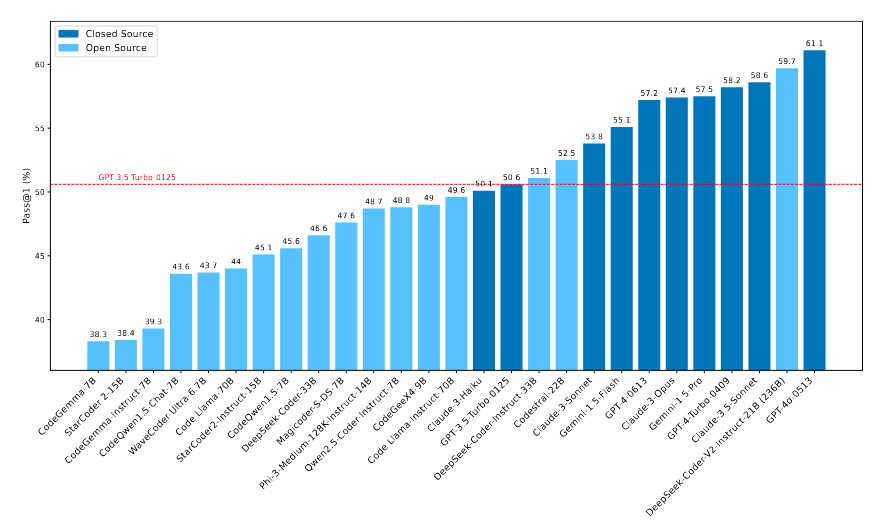
\includegraphics[width=0.8\textwidth]{./bilder/performance_comparison.png}
    \caption{Leistungsvergleich verschiedener Modellgrößen (nach Jiang et al. (2024), basierend auf 'A Survey on Large Language Models for Code Generation').}
    \label{fig:performance_comparison}
\end{figure}
In den letzten Jahren wurden mehrere Benchmarks und Evaluierungsdatensätze speziell für die Code-Generierung entwickelt. Beispiele dafür sind \emph{HumanEval}\cite{chen2021evaluatinglargelanguagemodels} und \emph{EvalPlus}\cite{evalplus}, die genutzt werden, um die Genauigkeit und Zuverlässigkeit von LLMs in verschiedenen Programmiersprachen zu testen. Erste Studien zeigen, dass LLMs einfache bis mittelschwere Aufgaben oft vollständig lösen können. Bei komplexeren oder sehr speziellen Aufgabenbereichen stoßen sie aber noch an ihre Grenzen\cite{NEURIPS2023_43e9d647}.
Obwohl LLMs in vielen Sprachen Code generieren können, hat sich Python als einer der Hauptfoki herauskristallisiert. Dies liegt an der weit verbreiteten Nutzung von Python in Wissenschaft und Industrie, insbesondere in den Bereichen Datenanalyse und Machine Learning. Die umfangreichen Bibliotheken wie NumPy, pandas und scikit-learn sind Teil der Trainingskorpora, wodurch LLMs häufig in der Lage sind, Standardroutinen oder Bibliotheksfunktionen korrekt anzuwenden\cite{chen2021evaluatinglargelanguagemodels}.

\subsection{Einführung Python}
\label{sec:Python}
TODO: ausführlicher
\subsubsection{Bedeutung und Bibliotheken}
Python ist dank seiner Syntax, aktiven Community und vielen hilfreichen Bibliotheken eine der am weitesten verbreiteten Sprachen für Datenanalyse. Ein paar der wichtigsten Bibliotheken, die in der Datenanalyse verwendet werden, sind:
\begin{itemize}
    \item \textbf{pandas} -- Datenstrukturen und -bearbeitung,
    \item \textbf{NumPy} -- numerische Berechnungen,
    \item \textbf{scikit-learn} -- Machine-Learning-Algorithmen,
    \item \textbf{Matplotlib} -- Visualisierung,
\end{itemize} 
Diese und weitere Bibliotheken ermöglichen eine effiziente Umsetzung datenanalytischer Projekte und werden bereits in LLM-Trainings berücksichtigt, wodurch generierter Code auf bekannte Funktionen zurückgreifen kann\cite{evalplus,chen2021codex}.

\subsubsection{Typische Schritte einer Datenanalyse}
Die Grundschritte einer klassischen Datenanalyse in Python enthält folgende Schritte:
\begin{enumerate}
    \item \textit{Datenimport} (z.\,B. CSV-Dateien, Datenbanken, APIs),
    \item \textit{Datenbereinigung} (fehlende Werte, Duplikate, Datentypen),
    \item \textit{Analyse und Visualisierung} (Statistiken, Plots),
\end{enumerate}
Im Rahmen dieser Arbeit wird untersucht, ob LLMs diese Schritte automatisieren können und an welchen Stellen manuell eingegriffen werden muss.

\subsection{Einführung automatisierte Code-Generierung}
\label{sec:AutoCode}

\subsubsection{Funktionsweise und Vorteile}
Automatisierte Code-Generierung mithilfe von LLMs basiert auf \emph{Prompts}, also Benutzeranfragen in natürlicher Sprache. LLMs haben hierbei die Möglichkeit sich flexibel an den vom Benutzer gegegeben Kontext anzupassen und können die natürliche Sprache in funktionsfähigen Code umwandeln. Ebenso müssen LLMs nicht spezifisch auf eine Aufgabe trainiert werden, aufgrund der großen Trainingsdaten, die ihnen zur Verfügung stehen\cite{chen2021evaluatinglargelanguagemodels}. Insbesondere für datenanalytische Aufgaben, bei denen standardisierte Skripte (z.\,B. für das Einlesen und Bereinigen von Daten) immer wieder benötigt werden, kann dies zu einer erheblichen Zeitersparnis führen und ermöglicht die Nutzung von LLMs auch für weniger erfahrene Personen, die nicht über tiefgreifende Programmierkenntnisse verfügen.

\subsubsection{Herausforderungen und Grenzen}
Trotz beeindruckender Fortschritte stößt die automatisierte Code-Generierung noch häufig an Grenzen\cite{nijkamp2023codegenopenlargelanguage,wang2021codet5identifierawareunifiedpretrained}:
\begin{itemize}
    \item \textbf{Komplexe Datenstrukturen}: LLMs zeigen teils Schwächen bei Aufgaben mit hochgradiger Komplexität oder spezifischem Wissen, wenn zu wenig Kontext durch den Nutzer gegeben wird\cite{nijkamp2023codegenopenlargelanguage,wang2021codet5identifierawareunifiedpretrained}.
    \item \textbf{Performanz}: Generierter Code ist nicht immer optimal hinsichtlich Laufzeit oder Speicherverbrauch\cite{wang2021codet5identifierawareunifiedpretrained}.
    \item \textbf{Wartbarkeit}: Kommentare, klare Code-Struktur und Dokumentation fehlen häufig.
    \item \textbf{Fehleranfälligkeit}: Auch Code, der vorerst funktionsfähig erscheint, kann immer noch Bugs oder Sicherheitslücken enthalten.
\end{itemize}
Wir präsent diese Herausforderungen in datenanalytischen Aufgaben sind, soll in den folgenden Kapiteln untersucht werden. Vor allem durch den Vergleich von generiertem und manuell geschriebenem Code lassen sich die Stärken und Schwächen von LLMs in der Datenanalyse besser einschätzen.

\section{LLMs in der Programmierung – aktueller Stand}
\label{sec:llms_programmierung}
Die Entwicklung von Large Language Models (LLMs) hat in den letzten Jahren nicht nur die Art und Weise, wie natürliche Sprache verarbeitet und generiert wird, verändert, sondern auch große Fortschritte in der automatisierten Code-Erstellung ermöglicht. Durch die Kombination aus leistungsstarken Modellarchitekturen wie Transformers, großen Mengen an Trainingsdaten und moderner Hardware haben LLMs heute eine große Präsemz in vielen Bereichen der Softwareentwicklung und Datenanalyse.
In diesem Kapitel werden die aktuellen Entwicklungen und verfügbaren Modelle vorgestellt. Außerdem wird ein Überblick über ihre Einsatzmöglichkeiten in der Softwareentwicklung und Datenanalyse gegeben. Zum Schluss werden wichtige Studien und Arbeiten zur Code-Generierung betrachtet, darunter etwa die von Chen et al. (2021) vorgestellte Arbeit zu Codex, einem Modell, das speziell für die automatisierte Programmierung entwickelt wurde\cite{chen2021evaluatinglargelanguagemodels} und die von Liu et al. (2023) veröffentlichte Arbeit zur Evaluation von generiertem Code mithilfe von \emph{EvalPlus}\cite{NEURIPS2023_43e9d647}.

\subsection{Überblick und Vergleich von verschiedenen LLMs}
Derzeit existiert eine Vielzahl an LLMs, darunter auch viele, die gezielt zur Code-Generierung entwickelt wurden. Zu den bekanntesten Beispielen zählen ChatGPT (GPTo1 als das modernste Modell), OpenAI Codex, Code Llama\cite{rozière2024codellamaopenfoundation}, StarCoder \cite{li2023starcodersourceyou}, CodeT5\cite{wang2021codet5identifierawareunifiedpretrained} oder CodeGen\cite{nijkamp2023codegenopenlargelanguage}.
\begin{figure}[H]
    \centering
    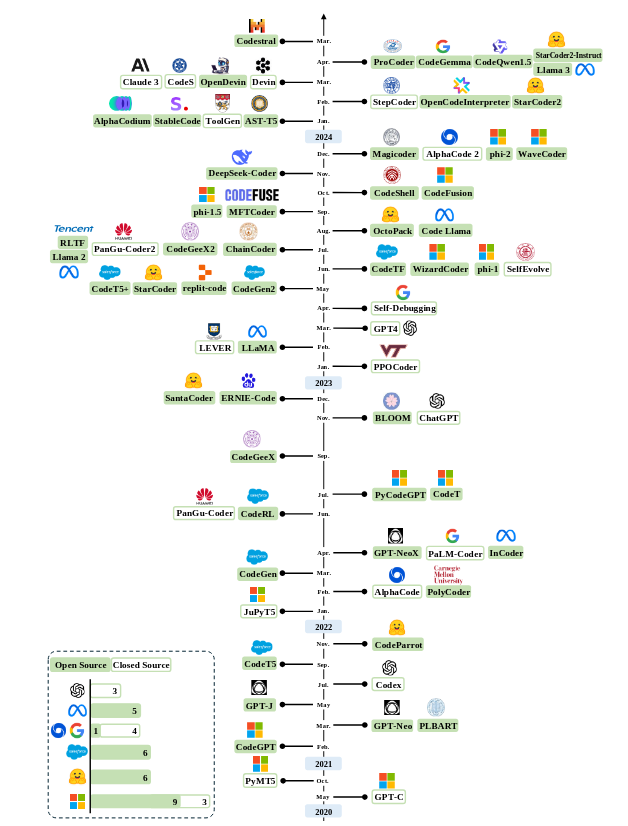
\includegraphics[width=0.8\textwidth]{./bilder/LLMs_for_coding.png}
    \caption{Chronologische Übersicht von Large Language Models für die Code Generierung der letzten Jahre (nach Jiang et al. (2024), basierend auf 'A Survey on Large Language Models for Code Generation').}
    \label{fig:llms_for_coding}
\end{figure}

Diese Modelle teilen sich häufig folgende Merkmale:
\begin{enumerate}
    \item \textbf{Transformer-Architektur}: Nahezu alle modernen LLMs beruhen auf dem Transformer-Modell.
    \item \textbf{Große Parameteranzahl}: Typische LLMs verfügen über eine Vielzahl an Parametern und benötigen entsprechend umfangreiche Trainingsdaten, zu denen in vielen Fällen öffentlich verfügbare Code-Repositories (z. B. GitHub) zählen\cite{chen2021evaluatinglargelanguagemodels}.
    \item \textbf{Breite Sprachenunterstützung}: Neben Python werden häufig Java, JavaScript und andere Programmiersprachen abgedeckt\cite{chen2021evaluatinglargelanguagemodels,jiang2024surveylargelanguagemodels}.
\end{enumerate}
Ein Vergleich der LLMs lässt sich anhand verschiedener Kriterien vornehmen:
\begin{itemize}
    \item \textbf{Größe und Trainingsdaten}: Modelle wie GPT-4 oder Code Llama sind mit einer Vielzahl an Code-Datensätzen trainiert und erreichen dadurch in Benchmarks eine hohe Erfolgsquote\cite{NEURIPS2023_43e9d647}.
    \item \textbf{Lizenz und Offenheit}: Neben proprietären Modellen, wie GitHub Copilot und ChatGPT, existieren mit Code Llama, StarCoder oder CodeGen auch Open Source Alternativen.
    \item \textbf{Spezialisierung}: Einige Modelle sind speziell auf Code-Generierung abgestimmt (z.B. Code Llama, StarCoder), wohingegen andere (z.B. ChatGPT) einen generellen Sprachkontext haben, um auch andere Fragen zu beantworten, der sich jedoch auch auf Code-Aufgaben anwenden lässt.
\end{itemize}

\subsection{Einsatzgebiete von LLMs in der Programmierung}
\label{sec:einsatzgebiete}
Die zunehmende Leistungsfähigkeit von Large Language Models (LLMs) ermöglicht es, Programmieraufgaben in diversen Bereichen zu automatisieren oder zu beschleunigen. Häufig genannte \emph{Einsatzgebiete} sind dabei:
\begin{itemize}
    \item \textbf{Code-Generierung}:
    Ermöglicht die Code-Generierung auf Grundlage von Beschreibungen aus natürlicher Sprache\cite{chen2021evaluatinglargelanguagemodels}. Ebenso bieten manche Modelle die Möglichkeit zu fertigen Funktionen Tests zu generieren, um dessen Funktionalität zu überprüfen.
    \item \textbf{Autovervollständigung}:  
    Integriert in Entwicklungsumgebungen wie Visual Studio Code können Tools wie GitHub Copilot repetitive Abläufe direkt im Code vervollständigen oder Vorschläge zur Vervollständigung von neu begonnenem Code liefern\cite{chen2021evaluatinglargelanguagemodels}.
    \item \textbf{Refactoring und Fehlersuche}:  
    Dank ihrer Kontextsensitivität können LLMs bestehenden Code analysieren und an einigen Stellen Möglichkeiten zur Optimierung oder Korrektur vorschlagen\cite{chen2021evaluatinglargelanguagemodels,wang2021codet5identifierawareunifiedpretrained}. Dadurch lassen sich Bugs, Redundanz und ineffiziente Code-Strukturen frühzeitig identifizieren und beheben.
    \item \textbf{Automatisierte Dokumentation und Code-Kommentierung}:  
    Viele Modelle bieten die Möglichkeit vorhandenen Code zu analysieren und dazu Kommentarblöcke oder gar ganze Dokumentationen zu erstellen\cite{wang2021codet5identifierawareunifiedpretrained,jiang2024surveylargelanguagemodels}.
\end{itemize}
Obwohl diese Einsatzgebiete großes Potenzial bieten, sind LLMs nicht frei von Fehlern. Gerade bei komplexen Entscheidungen zur Programm- und Codearchitektur können diese oft mit dem Level durch das menschliche Fachwissen nicht mithalten \cite{dhar2024llmsgeneratearchitecturaldesign}.

\subsection{Vergangene Studien und Arbeiten zur Code-Generierung}
\label{sec:vergangene_studien}

Die Forschung zur automatisierten Code-Generierung hat in den letzten Jahren eine rasante Entwicklung erlebt, wobei Arbeiten aus den Bereichen \emph{Software Engineering}, \emph{Large Language Models} und \emph{Machine Learning} zusammenfließen. Jiang et al. (2024) haben in ihrer Arbeit "A Survey on Large Language Models for Code Generation" eine Übersicht über die Entwicklung der veröffentlichten Arbeiten zu LLMs und Software Engineering erstellt, welche in Abbildung \ref{fig:entwicklung_paper} dargestellt ist.
\begin{figure}[H]
    \centering
    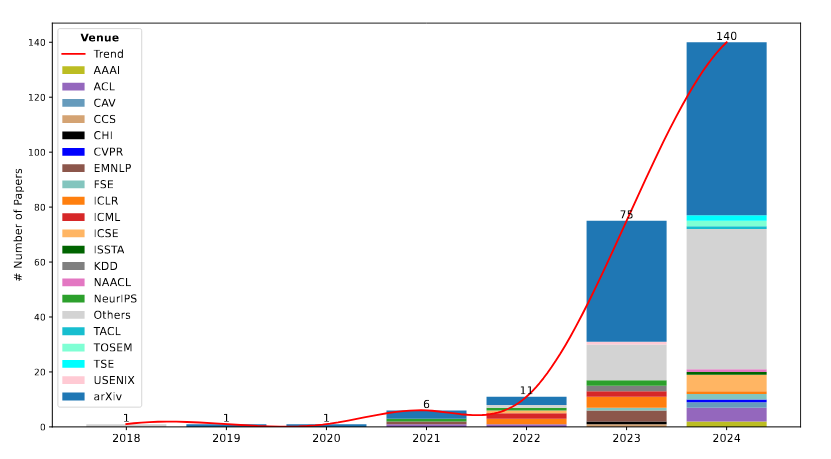
\includegraphics[width=0.8\textwidth]{./bilder/entwicklung_paper.png}
    \caption{Übersicht der Verteilung von veröffentlichten Arbeiten zu LLMs und Software Engineering der letzten Jahren (nach Jiang et al. (2024), basierend auf 'A Survey on Large Language Models for Code Generation').}
    \label{fig:entwicklung_paper}
\end{figure}

Im Folgenden werden einige vergangene Studien/Arbeiten zur Code Generierung mit LLMs vorgestellt:
\begin{enumerate}
    \item \textbf{"Is Your Code Generated by ChatGPT Really Correct? Rigorous Evaluation of Large Language Models for Code Generation"} von Liu et al. (2023) \cite{NEURIPS2023_43e9d647}:\\
    In diesem Paper wird untersucht, wie korrekt der von LLMs wie ChatGPT, Code Llama etc. generierte Code ist. Dafür wird \emph{EvalPlus} eingeführt. Dies ist ein neues Evaluierungsframework, das bestehende Testdatensätze wie \emph{HumanEval} durch weitere automatisierte Testfälle erweitert. Hier kommen Liu et al. zu dem Ergebnis, dass bisher viele Fehler in generiertem Code nicht erkannt wurden, wodurch die Modelle in ihrer Leistung überschätzt wurden. Die Autoren weisen darauf hin, wie wichtig umfassendene Tests sind, um die tatsächliche Funktionalität der LLMs für die Codegenerierung zu bewerten.
TODO: Vielleicht Grafik der Ergebnisse einfügen
    \item \textbf{Evaluating Large Language Models Trained on Code} von Chen et al. (2021) \cite{chen2021evaluatinglargelanguagemodels}:\\
    In diesem Paper wird Codex vorgestellt. Dies ist ein LLM, das speziell auf öffentlich verfügbarem Code von Github trainiert wurde, um dessen Fähigkeiten Python Code zu schreiben zu analysieren. Dies wird mithilfe des HumanEval-Datensatzes untersucht. Hierbei soll im genauen Python-Code aus Docstrings generiert und dieser dann bewertet werden. Die Ergebnisse zeigen, dass Codex im Vergleich zu anderen Modellen wie GPT-3 deutlich besser abschneidet, jedoch bei komplexeren Aufgaben seine Grenzen erreicht. Eine mehrfach wiederholte Lösungsgenerierung verbessert die Erfolgsrate, was das Potenzial ihres Ansatzes verdeutlicht.

    \item \textbf{A Survey on Large Language Models for Code Generation} von Jiang et al. (2024) \cite{jiang2024surveylargelanguagemodels}:\\
    Dieses Paper gibt einen allgemeinen und umfassenden Überblick über den aktuellen Forschungsstand zu LLMs für die Codegenerierung. Es greift Themen wie Datenaufbereitung, Modellarchitekturen und Benchmarks auf. Zudem werden Herausforderungen, wie die praktische Einführung und ethische Fragen diskutiert. Die Autoren leiten sich wichtige Forschungsfragen ab und verdeutlichen, dass LLMs in der Codegenerierung große Fortschritte gemacht haben, aber es weiterhin Potenzial zur Optimierung gibt.

    \item \textbf{Evaluating Language Models for Efficient Code Generation} von Liu et al. (2024) \cite{liu2024evaluating}
    Auch in dieser Arbeit von Jiawei Liu wird die Effizienz von Code untersucht, welcher von LLMs generiert wird. Hierbei mit Fokus auf Performance und Ressourcennutzung. Dafür wird \emph{Differential Performance Evaluation (DPE)} entwickelt und der \emph{EvalPerf}-Benchmark eingeführt. Dieser enthält komplexere Programmieraufgaben als der zuvor eingeführt \emph{EvalPlus}. Hier kommt man zu dem Entschluss, dass größere Modelle nicht automatisch auch effizienteren Code erzeugen. Stattdessen werden Effizienz und Korrektheit des Codes durch \emph{Instruction Tuning}(gezieltes Trainieren des Modells, um besser auf Anweisungen in natürlicher Sprache zu reagieren) verbessert.
\end{enumerate}
Zusammenfassend zeigen die genannten Studien, dass LLMs zwar großes Potenzial zur automatisierten Code Generierung besitzen, sie aber immer noch Probleme aufweisen und menschliche Entwickler nicht komplett ersetzen können. Besonders bei komplexeren Aufgaben, spezifischen Anforderungen oder Fragen zur Softwarearchitektur stoßen sie an ihre Grenzen.

\section{Methodik}
\label{sec:methodik}
TODO: noch mehr ausschreiben

\subsection{Vorgehensweise der Untersuchung}
    In der Untersuchung soll geprüft werden, inwieweit Large Language Models in der Lage sind gängige Datenanalyse-Schritte auf Grundlage eines gegebenen Datensatzes durchzuführen. Hierbei wird ChatGPT als aktueller Marktführer mit dem Sprachmodell GPTo1, welches das neueste Modell ist, verwendet. Ebenso gilt es herauszufinden wie qualitativ und effizient diese Lösung ist. Hierbei bezieht es sich auf die Forschungsfragen aus Kapitel \ref{sec:forschungsfragen}.
    Für die Vorgehensweise hierbei wird zuerst der verwendete Datensatz von Berlin Open Data an das Modell übergeben und dazu eine Prompt verfasst. Diese Prompts können in Kapitel \ref{sec:testfaelle} eingesehen werden.
    Im Anschluss durchläuft der Code mehrere Tests und manuelle Analysen um die Qualität und Effizienz des generierten Codes zu bewerten. Die genauen Auswertungskriterien sind in Kapitel \ref{sec:auswertungkriterien} aufgeführt.
    Die Ergebnisse der Auswertung werden in Kapitel \ref{sec:auswertung} detailliert dargestellt und auch mit den Ergebnissen anderer Arbeiten, wie etwa von Chen et al. (2021)\cite{chen2021evaluatinglargelanguagemodels} und Liu et al. (2023)\cite{NEURIPS2023_43e9d647} verglichen.

\subsection{Testfälle der Datenanalyse}
\label{sec:testfaelle}
\subsubsection{Testfall 1}
    Im ersten Testfall soll der Datensatz nach einer gewissen Spalte sortiert werden. Die Begründung hierfür ist, dass dies eine sehr einfache, aber auch sehr häufig aufkommende Datenanalyse-Aufgabe ist und somit einen guten Einstieg in die Untersuchung darstellt. Die Prompt für diese Aufgabe lautet: \emph{Hier ist meine CSV-Datei mit dem Namen "HZ\_2023.csv": \textbf{[CSV\_content]}, bitte analysiere diese Daten und erstelle mir ein Python Skript, das nach der Anzahl der Straftaten insgesamt eines Bezirks in 2023 sortiert.}.

\subsubsection{Testfall 2}
    Für den zweiten Testfall sollen die Tabellen der Excel Datei durch einen Join zusammengeführt und dann der Bezirk mit den meisten Straftaten insgesamt von allen Jahren kombiniert geliefert werden. Die Prompt für diese Aufgabe lautet: \emph{Erstelle mir ein Python Skript, mit welchem die Tabellen der Excel Datei durch einen Join zusammengeführt werden und der Bezirk mit den meisten Straftaten von allen Jahren kombiniert zurückgegeben wird.}.

\subsubsection{Testfall 3}
    Im dritten Testfall soll das Sprachmodell die prozentuale Verteilung der Straftaten in den Bezirken berechnen. Die Prompt für diese Aufgabe lautet: \emph{Erstelle mir ein Python Skript, mit welchem die prozentuale Verteilung der genauen Straftaten anteilig der Straftaten insgesamt pro Bezirk berechnet wird.}.

\subsubsection{Testfall 4}
    Im vierten Testfall soll eine simple Visualisierung des Datensatzes stattfinden. Es soll ein Balkendiagramm der Bezirke und der Verteilung der genauen Straftaten erstellt werden. Hierbei sollen die Bezirke auf der x-Achse und die Anzahl der einzelnen Straftaten mit ihrer Verteilung in einem Balken auf der y-Achse dargestellt und absteigend mit der Anzahl der Straftaten insgesamt pro Bezirk sortiert werden. Die Prompt für diese Aufgabe lautet: \emph{Erstelle mir ein Python Skript, mit welchem ein Balkendiagramm der Anzahl der Straftaten insgesamt und dessen Verteilung der genauen Straftaten pro Bezirk erstellt wird. Hierbei sollen auf der X-Achse die Bezirke und auf der Y-Achse pro Bezirk ein Balken über die Verteilung der Anzahl der Straftaten sein.}.

\subsubsection{Testfall 5}
    Für den letzten Testfall ist die Erstellung einer Zeitreihe vorgesehen. Hierbei soll die Anzahl der Straftaten insgesamt pro Jahr in einer Zeitreihe dargestellt werden. Die Prompt für diese Aufgabe lautet: \emph{Erstelle mir ein Python Skript, mit welchem eine Zeitreihe der Anzahl der Straftaten insgesamt pro Jahr dargestellt wird.}.


\subsection{Auswertungskriterien}
\label{sec:auswertungskriterien}
    Korrektheit des Codes und der Ergebnisse, Performance des Codes im Bezug auf Laufzeit und Ressourcennutzung, Qualität des Codes (Struktur des Codes, Kommentare/Dokumentation, verwendete Libraries), Wartbarkeit und ist der Code erweiterbar.\\

    Die Auswertung der generiertes Python Skripte erfolgt anhand der in Kapitel \ref{sec:forschungsfragen} definierten Kriterien. Um die Korrektheit des Codes zu messen wird das Pass@k Verfahren verwendet, dabei steht "k" für die Anzahl der ausgeführten Versuche pro Testfall. In diesem Experiment beschränke ich mich auf k=10, um eine gute Balance zwischen Genauigkeit und Rechenzeit zu finden. Bei diesem Verfahren ergibt sich als Ergebnis ein Prozentsatz über die Anzahl der erfolgreichen Versuche. Die ausgeführten Versuche werden anschließend in erfolgreich und nicht erfolgreich unterteilt und getrennt genauer betrachtet. Um zu entscheiden, ob ein Versuch erfolgreich war, werden Tests definiert, welche das Ergebnis und den Code selbst prüfen. Im Code wird dabei darauf geachtet, welche Bibliotheken, Funktionen und Pandas Dataframes benutzt wurden.
    In der genaueren Analyse des Codes wird bei den nicht erfolgreichen Versuchen wird untersucht, warum der Code nicht korrekt ausgeführt wurde und was für Verbesserungen vorgenommen werden können. Bei den erfolgreichen Versuchen hingegen wird analysiert, wie der Code strukturiert ist, ob er gut dokumentiert ist, ob er erweiterbar ist und wie die Laufzeit und Ressourcennutzung des Codes abschneidet.

\subsection{Verwendete Tools}
    \begin{enumerate}
        \item \textbf{Large Language Model}: Als Large Language Model wird ChatGPT mit GPTo1-mini verwendet, da ChatGPT als aktueller Marktführer gilt und GPTo1-mini das neueste und leistungsfähigste Modell ist, welches mit der OpenAI API verfügbar ist.
        
    \end{enumerate}

\section{Auswertung der Python-Code-Generiung zur Datenanalyse durch LLMs}
\label{sec:auswertung}

\section{Fazit und Ausblick}
\label{sec:fazit}

\newpage
% Literatur
\section{Literaturverzeichnis}
\label{sec:anhang}
\printbibliography
TODO: Abbildungsverzeichnis einfügen
\end{document}
